\documentclass{article}
\usepackage[utf8]{inputenc}
\usepackage{hyperref}
%\definecolor{linkcolour}{rgb}{0,0.2,0.6}
\usepackage{color}
\usepackage{float}
\usepackage{array}
\usepackage{booktabs}
\usepackage{xcolor} %for more colours to use in hyperref
\usepackage{graphicx}
\graphicspath{{Images/}}
\hypersetup{
    colorlinks=true, %set true if you want colored links
    linkcolor=forestgreen,
    citecolor={blue!50!black},
    urlcolor={blue!80!black}
    }
    
\usepackage{biblatex}

\addbibresource{ref.bib}    

\usepackage{titlesec}

\setcounter{secnumdepth}{4}

\titleformat{\paragraph}
{\normalfont\normalsize\bfseries}{\theparagraph}{1em}{}
\titlespacing*{\paragraph}
{0pt}{3.25ex plus 1ex minus .2ex}{1.5ex plus .2ex}    

\title{Automated Evaluation of Programming Assignments \\ \vspace{0.5mm} \large\textit{Related Papers}}
\author{Rishabh Manoj}
\date{\today}

\begin{document}

\maketitle

\section{A System to Grade Computer Programming Skills using
Machine Learning \cite{KDD}} 

Paper presents a method to grade assignments automatically using ML techniques at it's core. 

\begin{itemize}
    \item A novel grammar of features which captures signature elements in a program that human experts recognize when assigning a grade. In essence,
these features capture the functionality of the program. We show these features to correlate well with a proposed problem-independent rubric.\\

    \item Empirically shows that the novel features add value by better modeling human-grading than an elementary keyword-counts model.\\

\end{itemize}



  \begin{table}
    \centering% This is an environment - we probably don't want the extra spacing of center in addition to that added by table etc.
    \caption{Table of Scores and Characteristics}

    \small
    \begin{tabular}{*{2}{p{.425\linewidth}}}% The target layout does not centre the text so we don't want \centering
      \toprule% nicer rules courtesy of booktabs - but then we need to drop the verticals 
      Score &  Characteristics \\\midrule% Note that there is no & before the first column - & only comes between columns so if you define n columns, you can have at most n-1 & symbols in any row
               & \textbf{Completely correct and efficient:}\\  
       5 & An efficient implementation of the problem using the right control structures, data-dependencies and consideration of nuances/corner conditions of the logic.  \\ \midrule% the p{} setting automatically lets these be multi-line - we don't want multiple rows on top of that and this is simpler as TeX does the hard work for us
       
              & \textbf{Correct with silly errors:}\\
      4 & Correct control structures and critical data-dependencies incorporated. Some silly mistakes fail the code to pass test-cases.\\ \midrule
      
              & \textbf{Inconsistent logical structures:}\\
      3 & Right control structures exist with few/partially correct data dependencies.\\ \midrule
      
              & \textbf{Emerging basic structures:}\\
      2 & Appropriate keywords and tokens present, showing some understanding of a part of the problem.\\ \midrule
      
              & \textbf{Gibberish Code:}\\
      1 & Seemingly unrelated to the problem at hand.\\
      
      \bottomrule
    \end{tabular}
  \end{table}


\subsection{Features}

\paragraph{Basic Features:}
    The occurrences of various keywords and tokens
appearing in the source code like keywords related to control structures such as \textit{for, while, break, etc.}, operators defined by a language like '+','-','*', '\%', etc., character constants used in the program like '0', '1', '2', '100', etc., external function calls made like\textit{ print(), count(), etc.}\\

\textit{Reason:} Whether the right constructs even appear in a program (characteristics of Score 2 is present)

\paragraph{Expression Features:}
   The occurrences of expressions appearing in a program like explicit values, constants, variables, operators and functions.\\

\textit{Reason:} Help identify arithmetic and relational operations typical of the underlying algorithm.

\paragraph{Basic \& Expression Features in Control Context}
Occurrences of keywords and expressions with context (i.e) in a code block like loops, conditional-statements. Gets the control structures of the features described above.\\

\textit{Reason:} Characteristics of Score 3 

\paragraph{Data-Dependency Features}
Occurrence of particular kinds of expressions which are dependent on other particular kinds of expression. A data dependency is defined as any hierarchical ordering observed in the Data Dependency Graph (DDG) of the program.\\

\textit{Reason:} Value of one variable of an expression has influence on the variable of the other expression, which creates a hierarchy for expressions and assigning weightage to expression is easier.

\paragraph{Data-Dependency in Control Context}
Above thing with context.\\

\textit{Reason:} Gives more info on the hierarchy of expressions.\\

Point 4 \& 5 are crucial, explains whether the algo is correct, necessary conditions.\\

\textbf{\textit{Thoughts}
}\\
PDGs can be substituted for this? Need to research. Instead of comparing PDG through $\gamma$-isomorphism boil down to feature 4 \& 5 and do regression? clustering for approaches? Take PDG of all correct sol. and feed it to an SVM and attempt classification? 


\subsection{Machine Learning}

Attempted various methods like Linear Regression, Ridge Regression, SVM, Random Forests.\\

Results show Ridge Regression has the best results  with an average of 0.8 correlation.\\

Further insights of feature selection shows in some examples the most important feature selected as similar to one that a human would pick.\\ 

\textbf{\textit{Thoughts}}

Really Impressive. Humans usually evaluate by checking if the most important block of code is present. If possible to extract that by seeing all correct solutions then problem can be simplified by checking for blocks of code in order of importance and assigning grades.\\ 

Possible cons: Different approaches for problem might mess up the structure.\\ 

\section{Improving the Automatic Evaluation of Problem
Solutions in Programming Contests \cite{ribeiro2009improving}} 

The paper is specifically tailored for IOI programming contests but there are certain points that are useful.

One approach to assign grades is to look at the running time of the code. The authors set up solutions A,B \& C to the same problem with various complexities.

\begin{itemize}
    \item A --- $\mathcal{O}(N^3)$
    \item B --- $\mathcal{O}(N^2)$
    \item C --- $\mathcal{O}(N)$
\end{itemize}

They experimentally increased the value of N from low to high and plotted the graph of time taken to solve.

\begin{figure}[H]
    \centering
    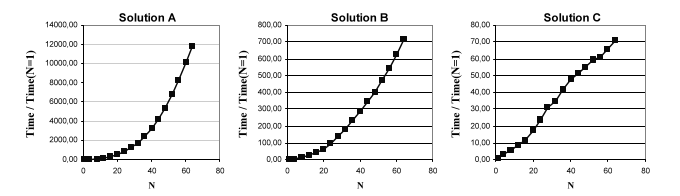
\includegraphics[height=1.2in]{Images/complexity_graphs.png}
    \caption{Comparative time spent for running the three implemented solutions as N linearly grows.}
\end{figure}

Using simple statistical method of taking the maximum correlation coefficient with various categories like $\log N$, $N$, $N^2$, $N^3$, $N^4$ $\cdots$, they calculate to which category the graph (aka solution) belong to.\\

\begin{figure}[H]
    \centering
    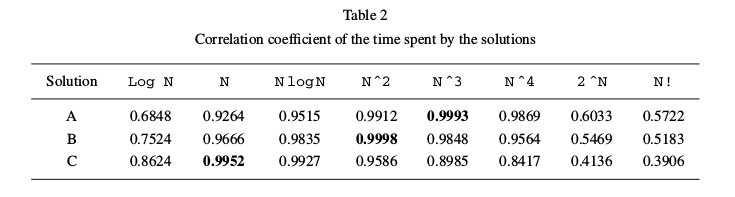
\includegraphics[height=1.2in]{table_corr_complexity.png}
    %\caption{Comparative time spent for running the three implemented solutions as N linearly grows.}
\end{figure}

\textbf{\textit{Thoughts}}

Instead of trying to classify the solution into one of the labels ($\log N,N,N^2,N^3$), we take note of the running time (as well as other entities like memory usage and other features of a program while running on test cases), add it as an attribute along with the boiled down PDG and feed it to an ML classifier.\\

Including both run time attributes as well as static attributes will maybe capture essential feature to cluster the correct solutions.\\

Possible cons: No impact on grading the incorrect solutions as running time cannot be calculated properly (Infinite loops, Program crash, etc...)
 
\section{Automated Feedback Generation for
Introductory Programming Assignments \cite{singh2013automated}}
(This was referenced in Jayendran's Thesis)\\

INCOMPLETE!!\\


The paper presents a method for automatically providing feedback. It uses a reference implementation of the assignment, and an error model consisting of potential corrections to errors that students might make to give feedback.\\

\begin{itemize}
    \item Paper uses Python as reference language, my understanding is that the model is specifically tailored to Python.

    \item It introduces a high level Error Model Language that provide correction rules

    \item Evaluated on real world and could provide feedback on 64\% of submitted solution in about 10 seconds. 
\end{itemize}


Uses some SKETCH tool to do something, Unclear!!.\\ 

//TODO Read about SKETCH and CEGIS algorithm before continuing!!\\


\textbf{\textit{Thoughts}}

EML has to be manually generated, seems infeasible for large scale usage? Unclear!!







\printbibliography

\end{document}
